%-----------------------------------------------------------------------------%
\chapter{\babTiga}
%-----------------------------------------------------------------------------%

%-----------------------------------------------------------------------------%
\section{Alur Penelitian}
%-----------------------------------------------------------------------------%
Dalam suatu penelitian, terdapat urutan tahapan yang perlu dilakukan. Alur penelitian ini mengandung seluruh langkah yang harus ditempuh, mulai dari fase perancangan hingga tahap akhir penelitian.
 \begin{figure}
	\begin{center}
		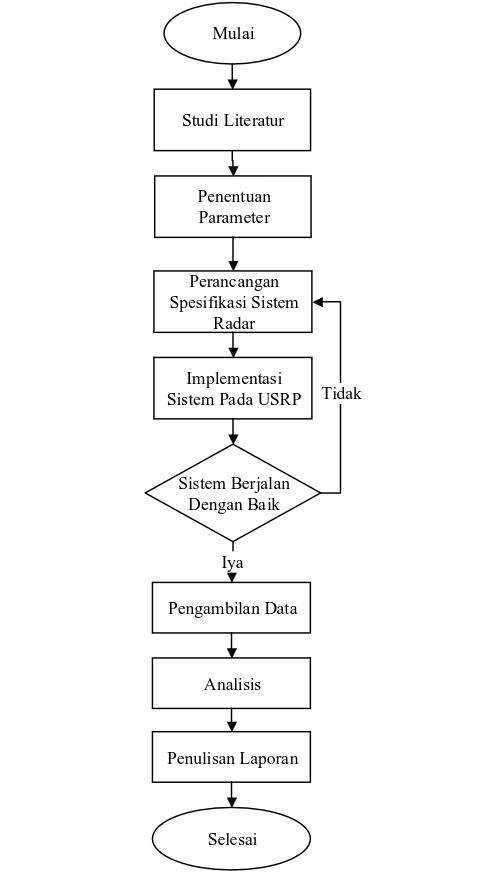
\includegraphics[scale=0.5]{pics/bab3/flowchart2.png} 
		\label{img:flowchart}
		\caption[\textit{Flowchart} Penelitian]{\textit{Flowchart} Penelitian}
	\end{center}
\end{figure}
Pada alur penelitian yang telah dirancang, terdapat 6 tahap yang perlu dilakukan setelah penelitian dimulai dan sebelum penelitian diakhiri. Tiap tahapan yang telah dirancang harus dilaksanakan sebaik mungkin agar hasil yang diharapkan dapat tercapai.


\section{Studi Literatur}
Pada tahap ini, dilakukan studi literatur terhadap masalah yang diangkat serta solusi yang diajukan pada proposal ini. Studi literatur meliputi kajian artikel terdahulu hingga kajian terhadap perangkat lunak yang digunakan serta metode yang dilakukan dalam penyelesaian masalah.
	
\section{Penentuan Parameter}

Pada tahap ini, parameter penelitian ditentukan, dengan parameter perancangan sebagai berikut.

\begin{center}
	\begin{longtable}{| c | c | c |}
		\caption{Parameter Penelitian}
		\label{tab:param}\\
		\hline
		No. & Parameter Penelitian 			& Satuan\\ \hline
		1.  &\textit{Center Frequency}	   	& GHz\\
		2.  &\textit{Bandwidth} 			& MHz \\
		\hline
	\end{longtable}
\end{center}

Sementara itu, untuk memastikan hasil yang dicapai baik, maka perlu ditentukan pula parameter pengujian, sebagai berikut.

\begin{center}
	\begin{longtable}{| c | c | c |}
		\caption{Parameter Pengujian}
		\label{tab:paramUji}\\
		\hline
		No. & Parameter Pengujian		& Satuan\\ \hline
		1.  &Jarak	   					& m\\
		2.  &Kecepatan 					& m/s\\
		3.  &\textit{RMSE}				& -\\
		\hline
	\end{longtable}
\end{center}

\section{Perancangan Spesifikasi Sistem}
Pada tahap ini, dilakukan perancangan tentang penelitian yang diangkat, dalam konteks ini adalah radar. Sehingga perlu dilakukannya penentuan spesifikasi radar berdasarkan perangkat keras yang digunakan. Penelitian ini menggunakan alat USRP berseri B210.  Spesifikasi dari alat ini akan dijelaskan pada tabel berikut.

\begin{center}
	\begin{longtable}{| c | c | c |}
		\caption{Spesifikasi Sistem Radar}
		\label{tab:spekRadar}\\
		\hline
		No. & Spesifikasi 					& Keterangan\\\hline
		1.  & USRP 							& B210\\
		2.  & \textit{Center Frequency}  	& 3 GHz \\
		3.  & \textit{Bandwidth} 			& 50 MHz \\
		4.	& Bentuk Modulasi				& \textit{Triangular}\\
		5.  & Jarak Maksimum 				& 150 km \\
		6.  & Resolusi Jarak 				& 3 m \\
		7.  & Kecepatan Maksimum			& 15 $m/s$ \\
		8.  & Resolusi Kecepatan 			& 1 $m/s$\\
		9.	& Durasi \textit{Chirp}			& 0.001667 s\\
		10.	& \textit{Chirp Rate}			& 30000 MHz\\
		\hline
	\end{longtable}
\end{center}

\begin{itemize}
	\item Hitung panjang gelombang ($\lambda$) dari frekuensi tengah yang sudah ditentukan yaitu 3 GHz.
	\begin{align*}
		\lambda &= \frac{c}{F_{c}}\\
		\lambda &= \frac{3 \cdot 10^{8}}{3 \cdot 10^{9}}\\
		\lambda &= 0.1 m
	\end{align*}

	\item Menghitung resolusi jarak berdasarkan persamaan \ref{eq:RangeRes} dan dengan menentukan \textit{bandwidth} bernilai 50 MHz, maka.
		\begin{align*}
			R_{res} &= \frac{c}{2 BW} \\
			R_{res} &= \frac{3 \cdot 10^{8}}{2 \cdot 50 MHz}\\
			R_{res} &= 3 m
		\end{align*}
	\item Menghitung jarak maksimum yang dapat dideteksi oleh radar digunakanlah persamaan \ref{eq:MaxRange}, namun sebelumnya harus ditentukan terlebih dahulu nilai $\mu$, yang merupakan tingkat kenaikan frekuensi pada suatu periode sesuai dengan persamaan \ref{eq:chirpRate}, dengan nilai $T_{c}$ sesuai persamaan \ref{eq:chirpTime} dan nilai kecepatan maksimum ditentukan bernilai 15 m/s, maka.
	
	\begin{align*}
		T_{c} &= \frac{\lambda}{4 \cdot V_{max}}\\
		T_{c} &= \frac{0.1}{4 \cdot 15}\\
		T_{c} &= 0.001667
	\end{align*}

	\item 
	Sehingga nilai $\mu$ dapat dihitung menjadi.

		\begin{align*}
		\mu &= \frac{\textit{Bandwidth}}{T_{c}}\\
		\mu &= \frac{\textit{50 MHz}}{0.001667}\\
		\mu &= 30000 MHz/s
		\end{align*}

	\item 	
	Dengan jarak maksimum yang didapat adalah.
		\begin{align*}
		R_{max} &= \frac{F_{s} \cdot c}{2 \cdot \mu}\\
		R_{max} &= \frac{30 \cdot 10^{6} \cdot 3 \cdot 10^{8}}{2 \cdot 30000}\\
		R_{max} &= 150 m
		\end{align*}

	\item 
	Dengan $T_{f}$ sebagai durasi \textit{frame} bernilai 0.05 s maka resolusi kecepatannya.
		\begin{align*}
			V_{res} &= \frac{\lambda}{2 \cdot T_{f}}\\
			V_{res} &= \frac{0.1}{2 \cdot 0.05}\\
			V_{res} &= 1 m/s
		\end{align*}

\end{itemize}

\section{Implementasi Sistem}
Tahap implementasi ini dilakukan pada aplikasi GNURadio dan menghasilkan \textit{flow diagram} yang merepresentasikan langkah yang dilakukan pada USRP. \textit{Flow diagram} yang didesain sudah memenuhi spesifikasi sistem radar pada tabel \ref{tab:spekRadar}. 

Implementasi sistem akan dilaksanakan pada beberapa perangkat, mulai dari laptop, antena, dan USRP. Berikut detail perangkat yang akan digunakan pada saat implementasi guna mendapat hasil yang baik.

\begin{enumerate}
	\item \textit{IdeaPad Gaming 3 15ARH7} :
	\begin{figure}
		\begin{center}
			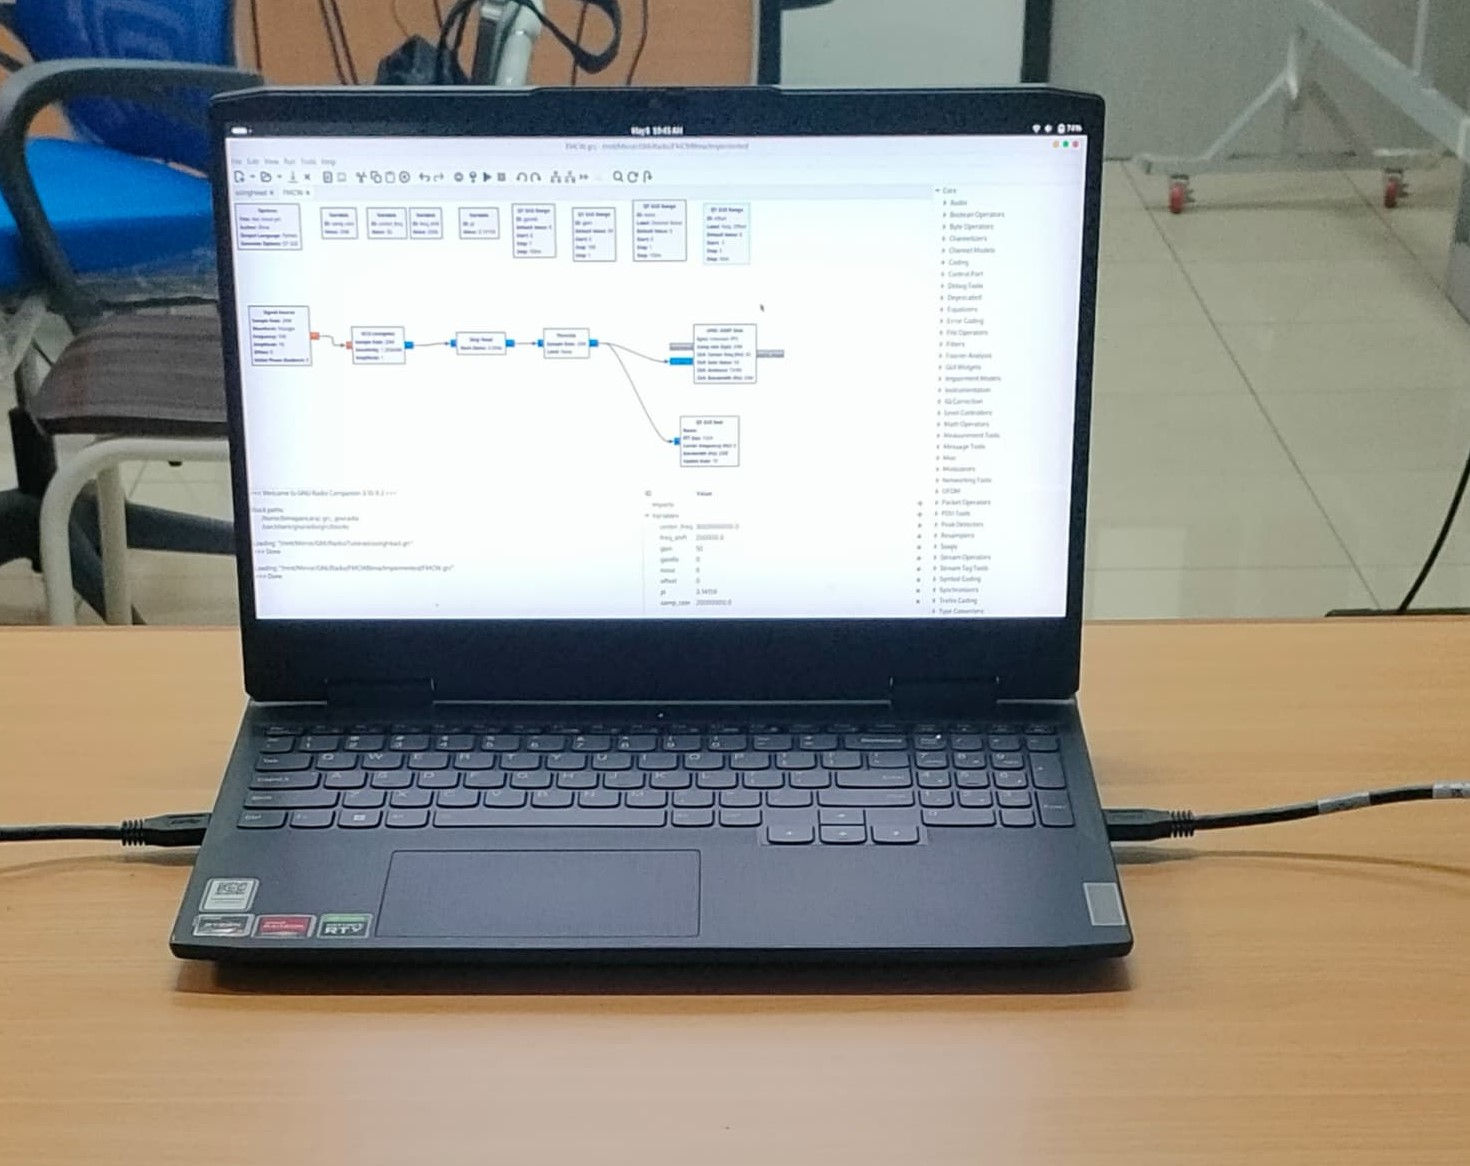
\includegraphics[scale=0.2]{pics/bab3/laptop.jpg} 
			\caption[Gambar Perangkat Laptop Yang Digunakan]{Gambar Perangkat Laptop Yang Digunakan}
			\label{pic:contohBlokGRC}
		\end{center}
	\end{figure}

	\begin{itemize}
		\item \textit{Processor} : AMD Ryzen 7 6800H dengan \textit{Radeon Graphics} 3.20 GHz
		\item \textit{Memory} : 8,00 GB (7,19 GB \textit{usable})
	\end{itemize}

	\item Perangkat \textit{Software Defined Radio} :
	\begin{figure}
		\begin{center}
			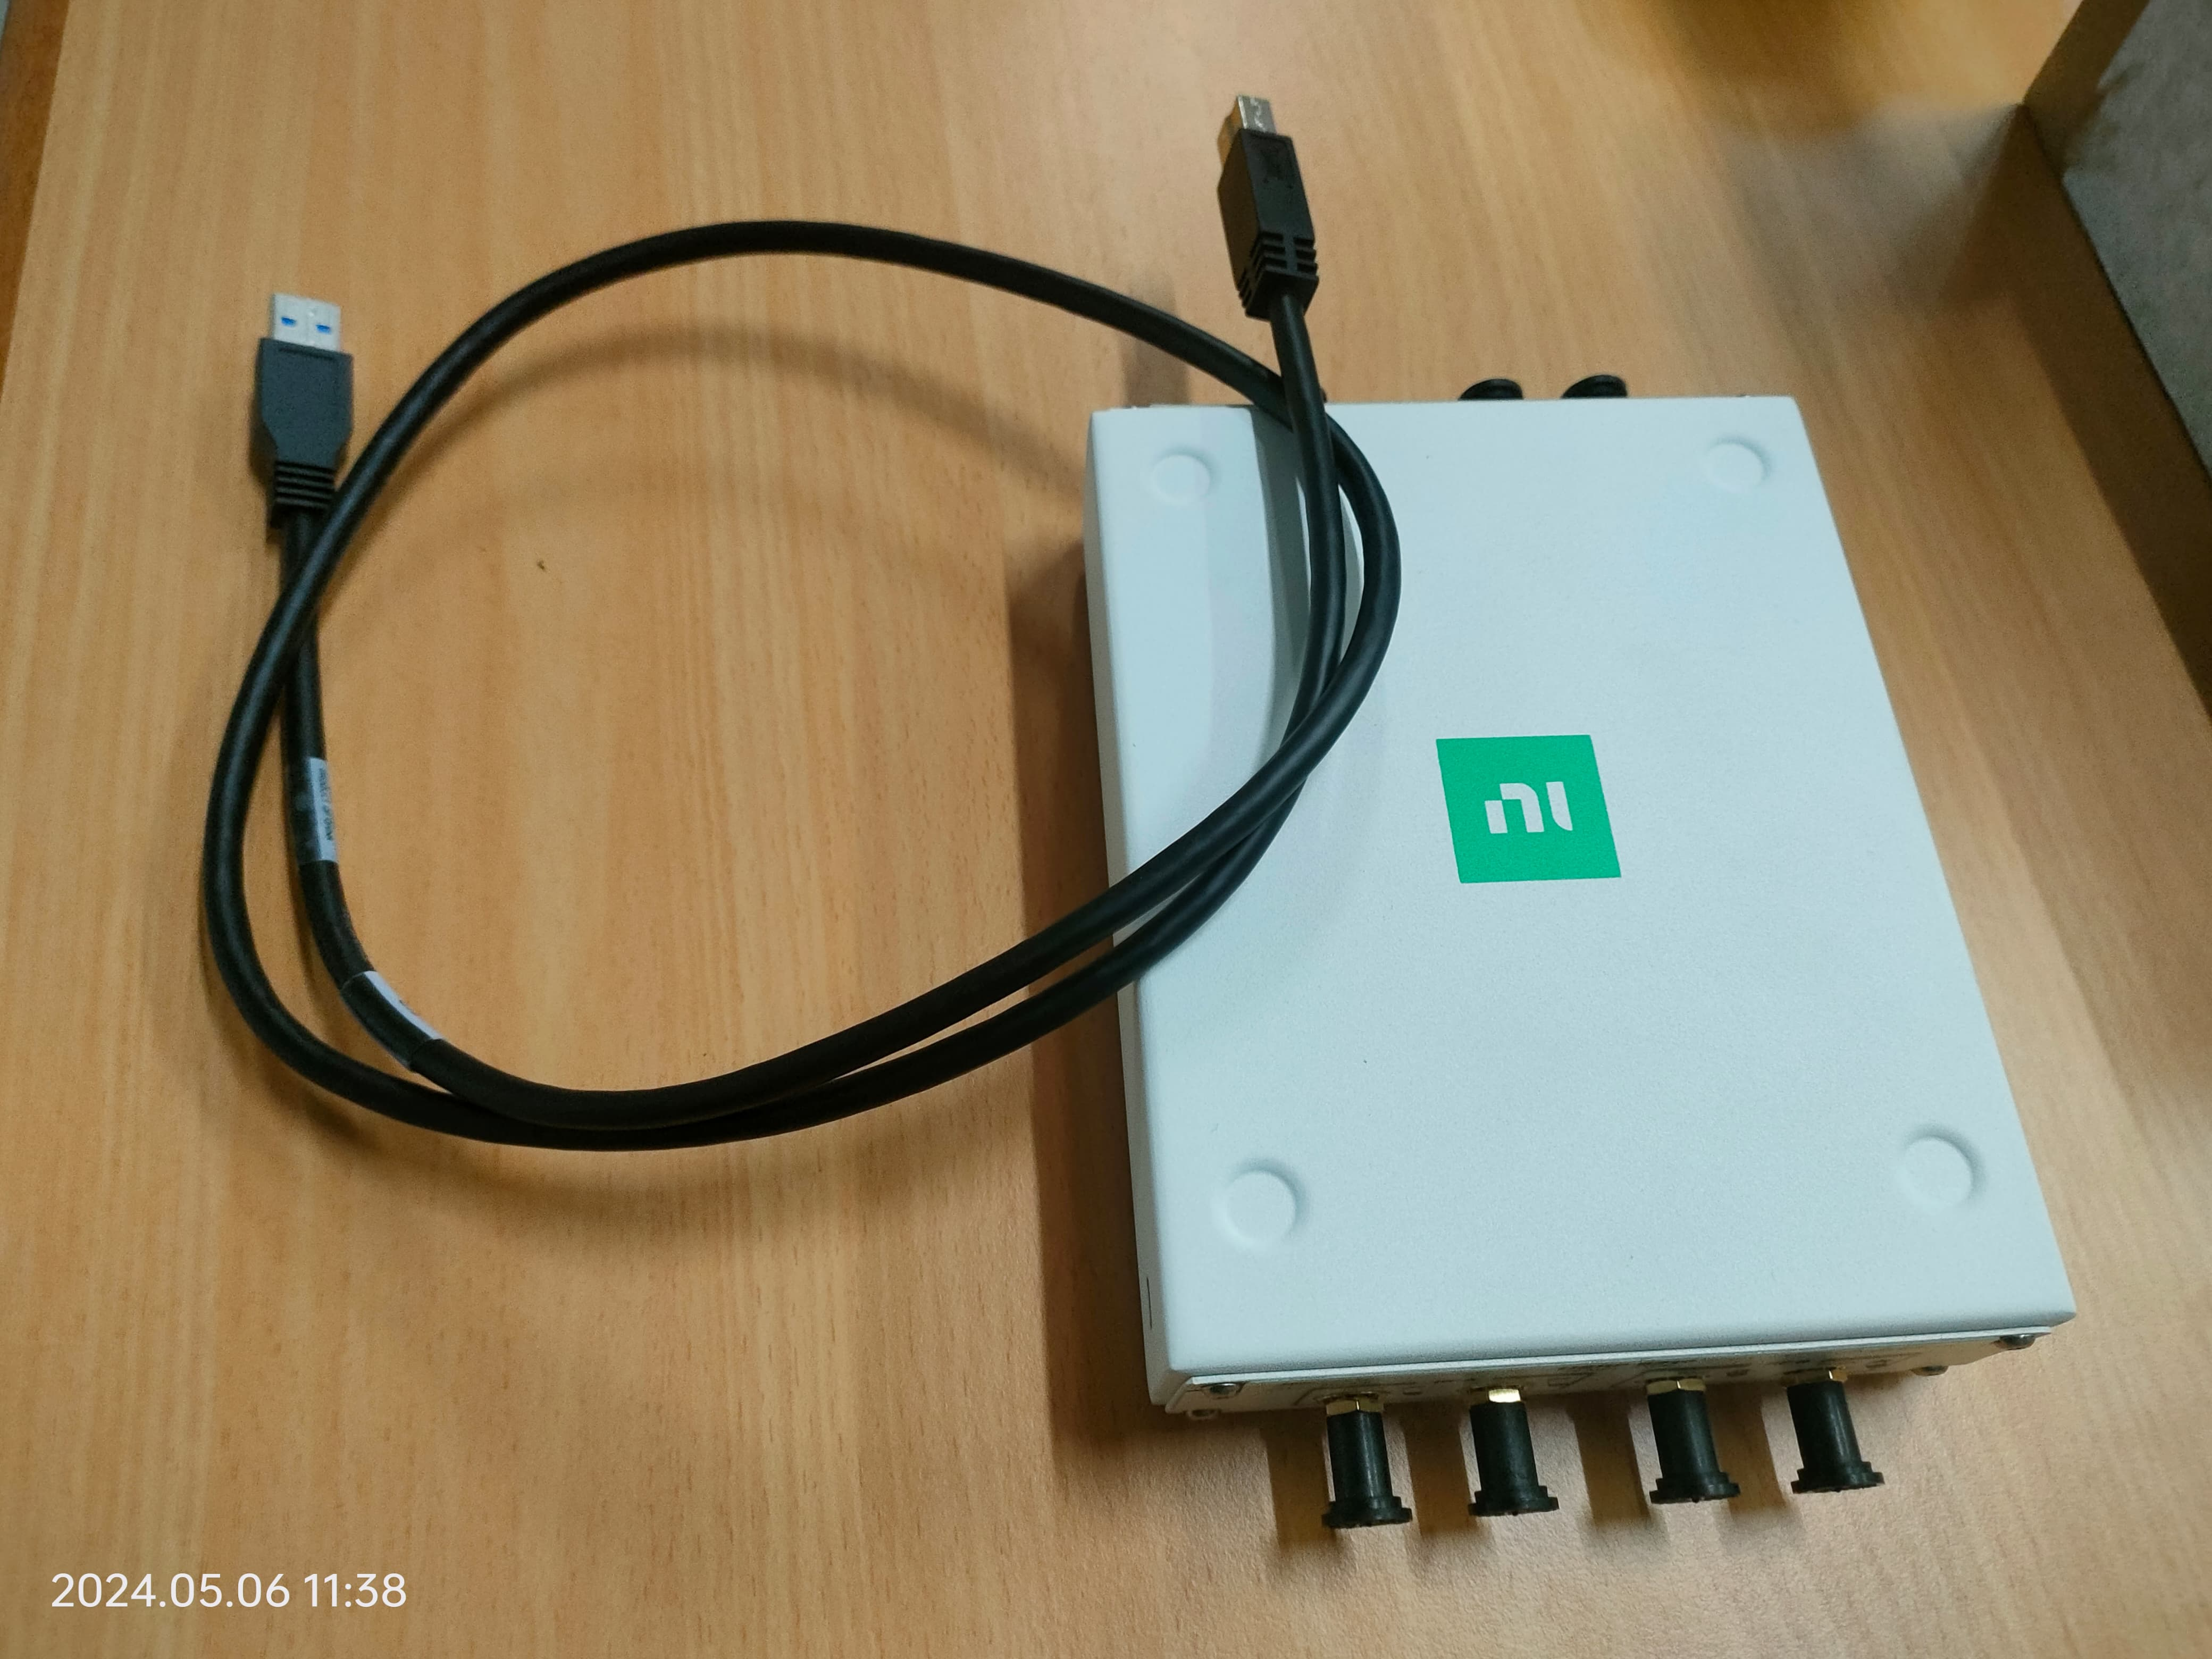
\includegraphics[scale=0.045]{pics/bab3/usrp2.jpg}
			\caption{Alat USRP B210}
			\label{img:logPeriodic}
		\end{center}
	\end{figure}
	\begin{itemize}
		\item Tipe : USRP B210 
		\item Jarak Frekuensi : 70 MHz - 6 GHz 
	\end{itemize}

	\item Antena \textit{Log-periodic} :
	\begin{figure}
		\begin{center}
			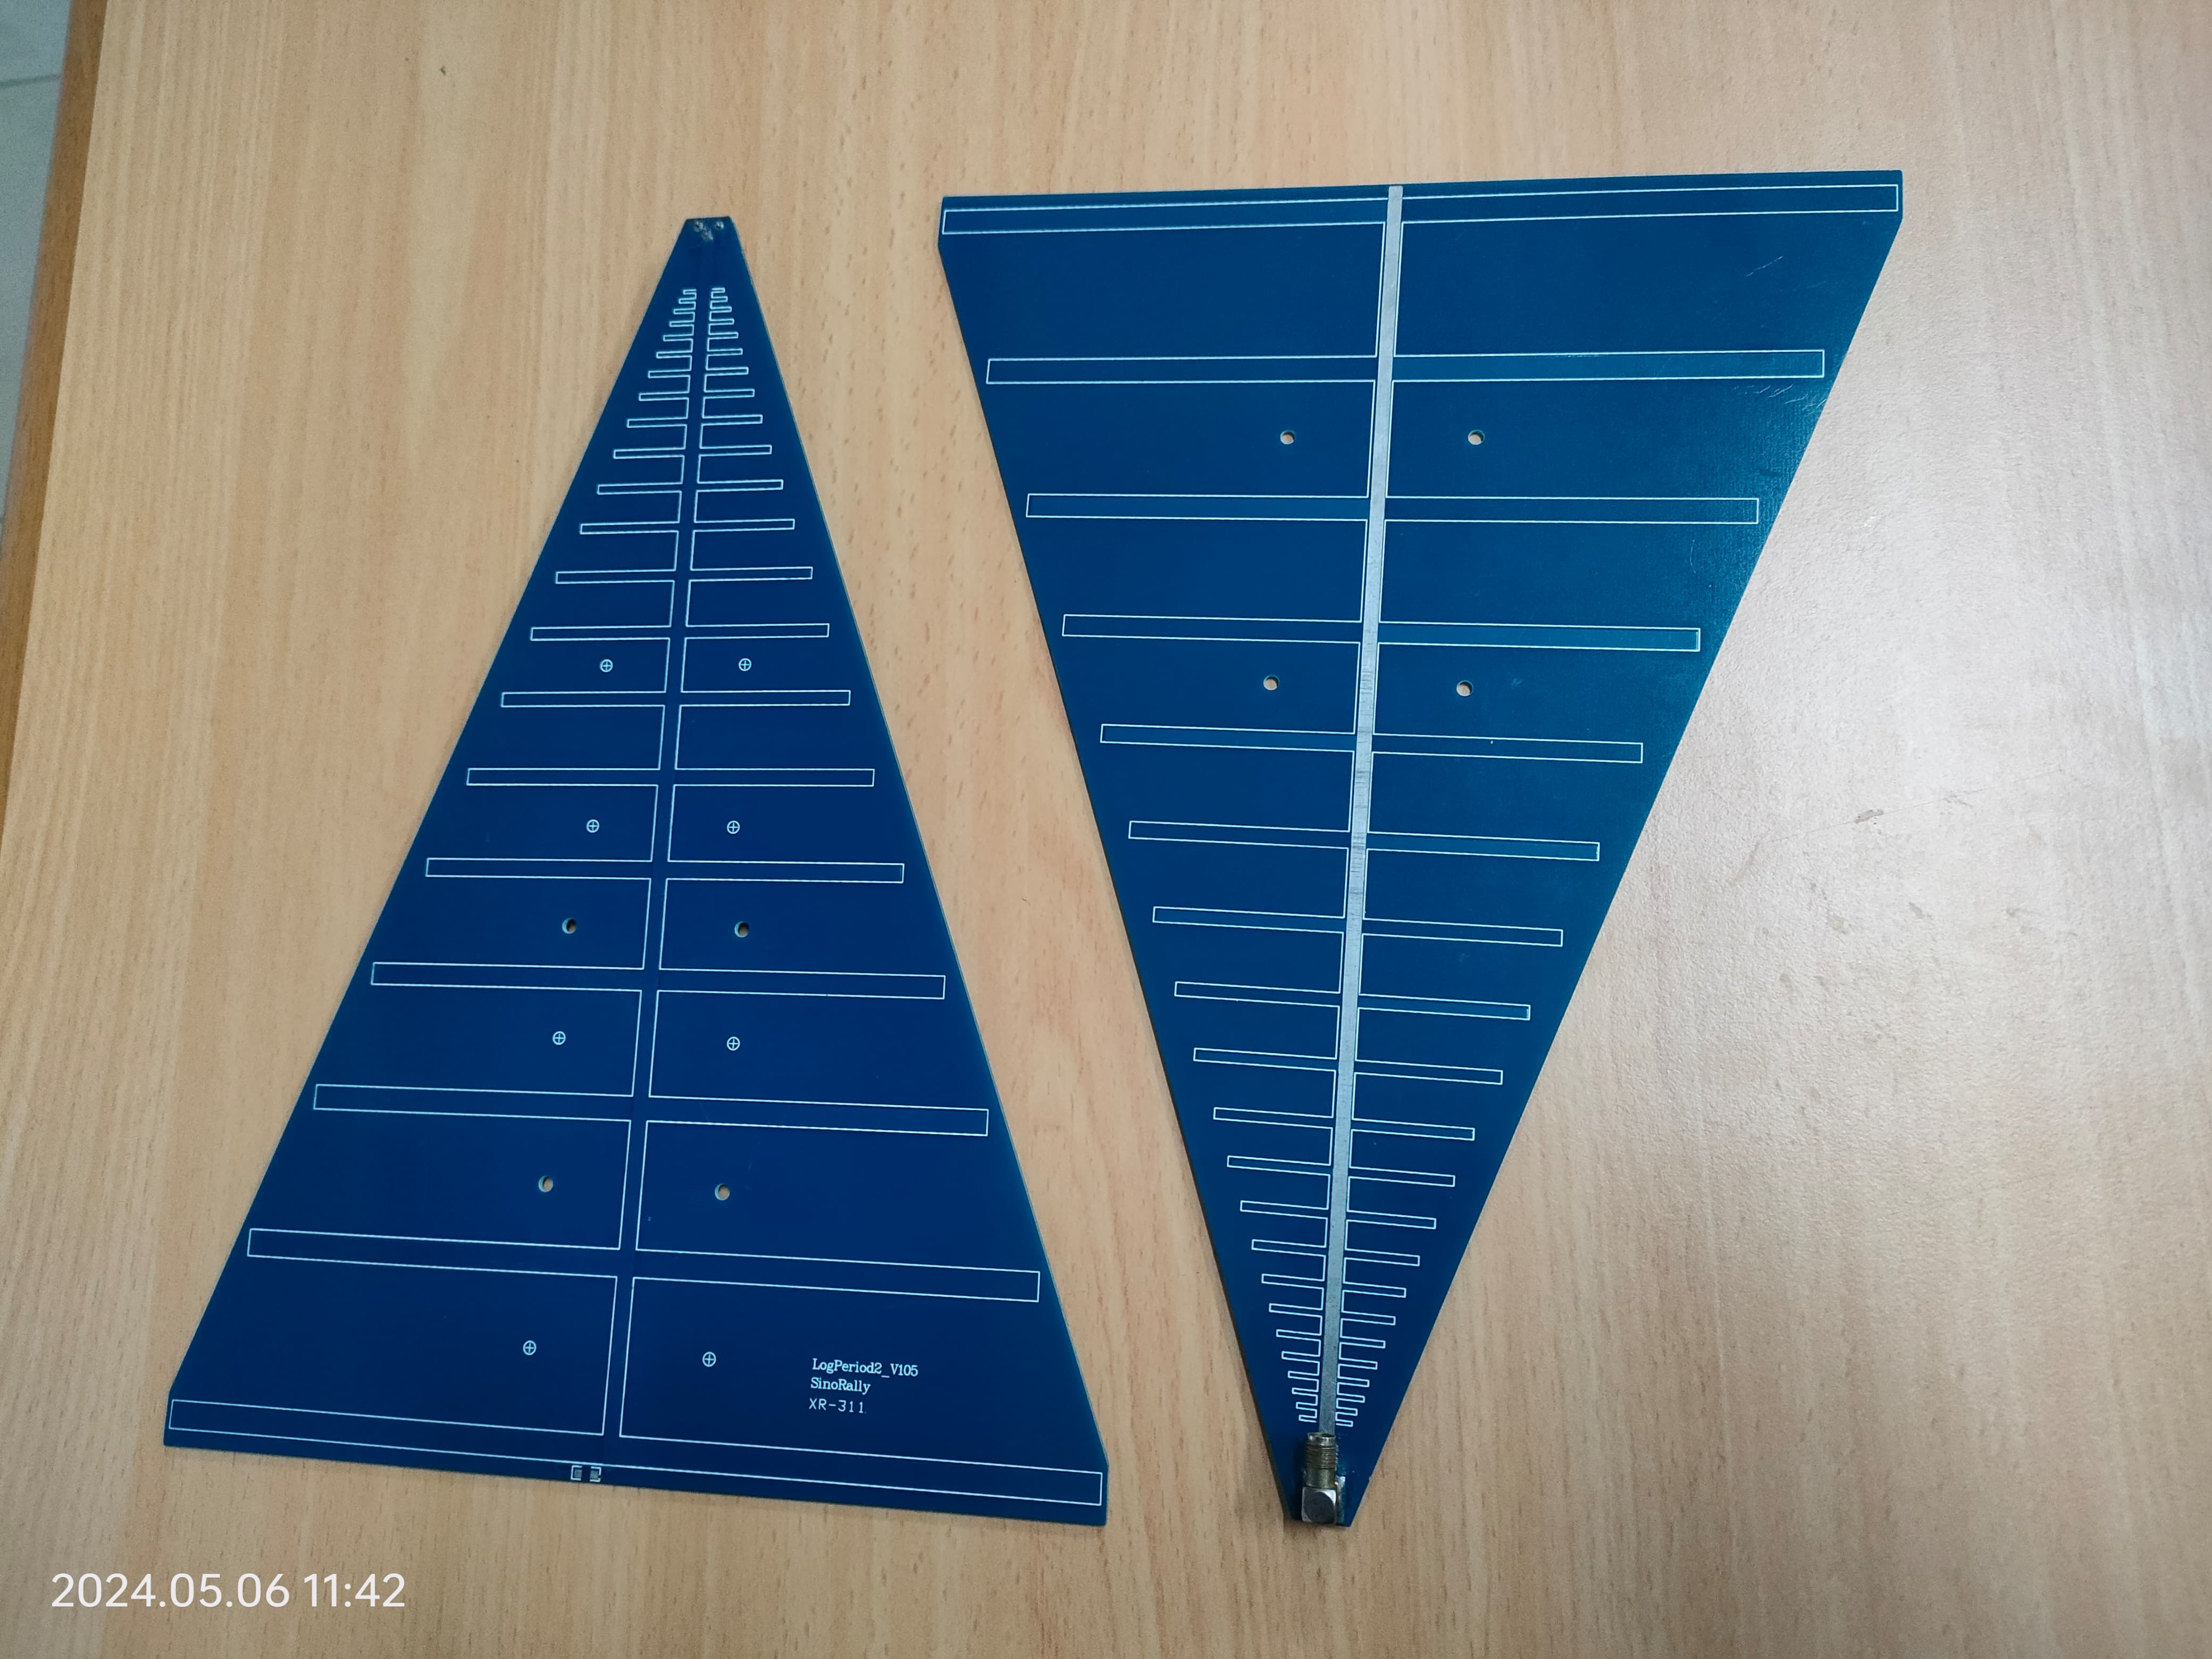
\includegraphics[scale=0.05]{pics/bab3/logPeriodic.jpg}
			\caption{Antena \textit{Log Periodic} Pengujian}
			\label{img:usrpBoard}
		\end{center}
	\end{figure}
	\begin{itemize}
		\item Frekuensi : 800 MHz - 6GHz 
		\item Pola Radiasi : \textit{Directional}
		\item \textit{Gain} : 5.2 - 6.3 dB
	\end{itemize}
\end{enumerate}

	
\section{Pengambilan Data}
Pada tahap ini, pengambilan data dengan radar yang sudah didesain dan diimplementasikan pada USRP dilakukan. Pengambilan data akan dilaksanakan di lokasi lapangan Univertitas Telkom Surabaya yang beralamat Jl. Ketintang No.156, Ketintang, Kec. Gayungan, Surabaya, Jawa Timur 60231.

\begin{figure}
	\begin{center}
		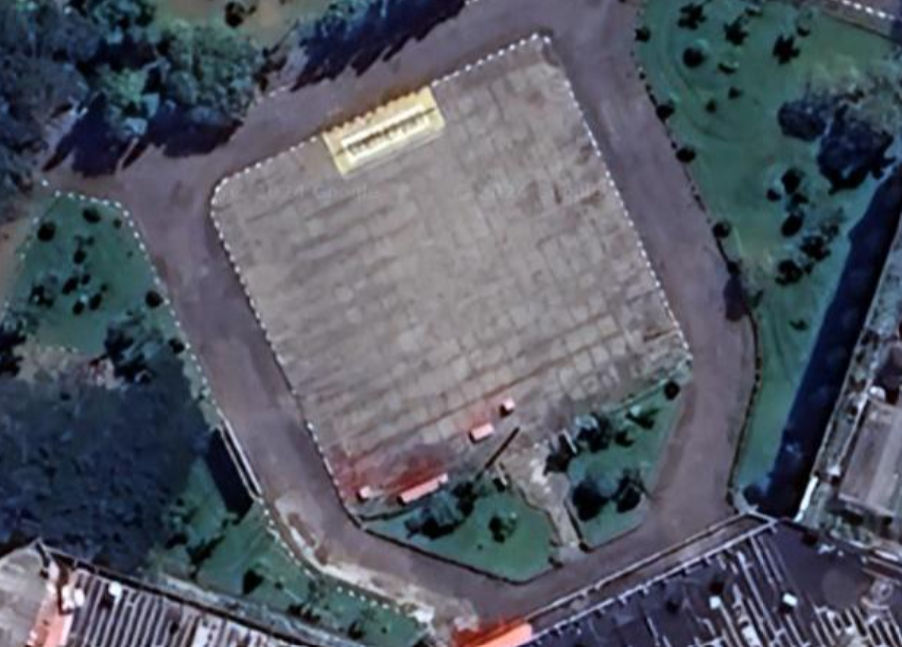
\includegraphics[scale=0.4]{pics/bab3/petaPengujian.png}
		\caption{Lokasi Pengujian}
		\label{img:petaUji}
	\end{center}
\end{figure}

Pengujian dilakukan dengan menggunakan kendaraan roda empat sebagai objek yang akan dideteksi. Dengan begitu, maka pengambilan data kecepatan dapat dilakukan dan dapat dibandingkan dengan hasil yang didapat dari radar yang telah didesain.

\begin{figure}
	\begin{center}
		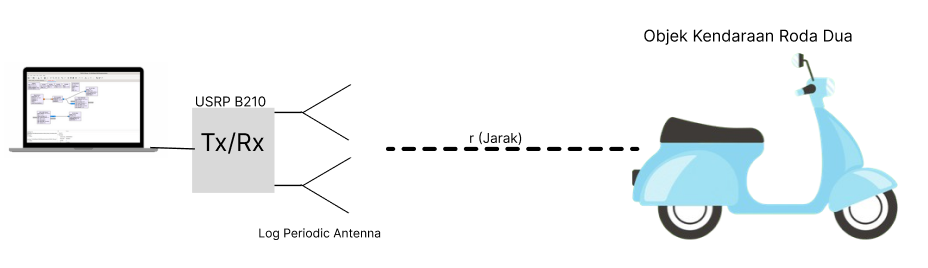
\includegraphics[scale=0.4]{pics/bab3/skema.png}
		\caption{Skema Penelitian}
		\label{img:skema}
	\end{center}
\end{figure}

\section{Konfigurasi Pengujian}
Konfigurasi pengujian dilakukan sesuai dengan gambar \ref{img:skema}. Terdapat satu buah perangkat laptop yang terhubung dengan dua buah USRP, masing-masing USRP terhubung dengan antena \textit{Log-periodic}. USRP 1 berperan sebagai \textit{transmitter} sedangkan USRP 2 berperan sebagai \textit{receiver}.

\begin{figure}
	\begin{center}
		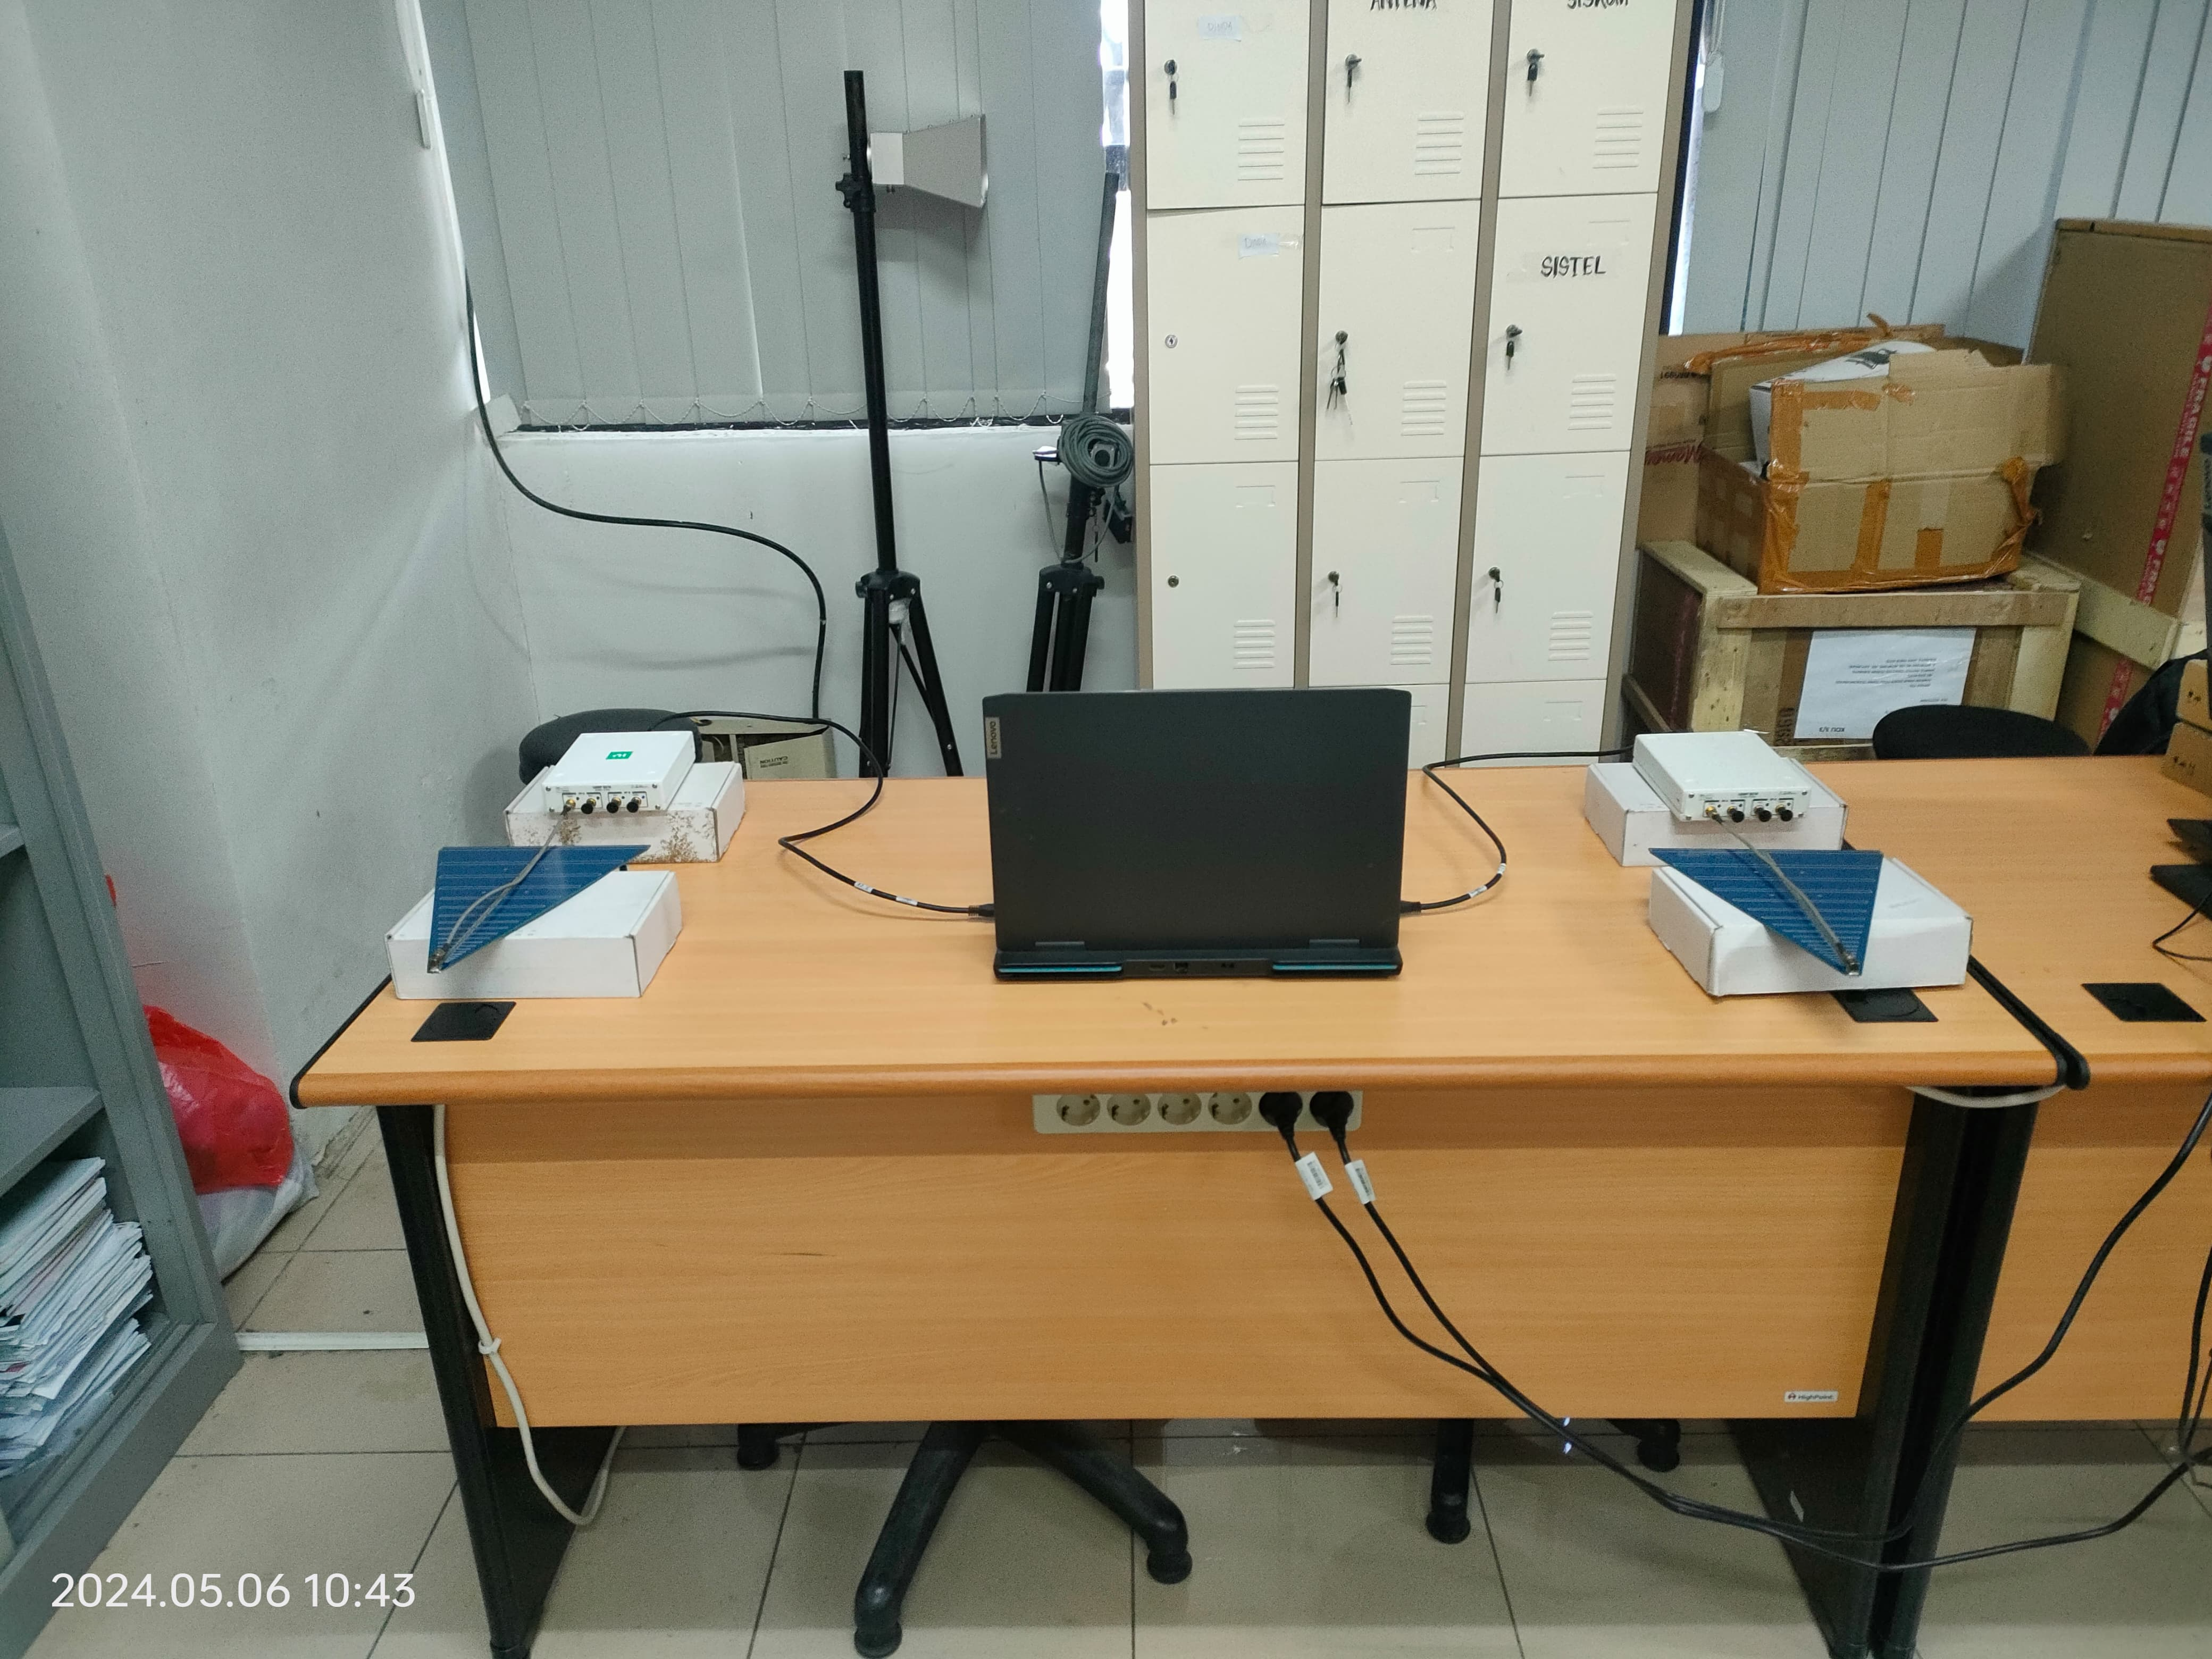
\includegraphics[scale=0.09]{pics/bab3/konfigurasiPengujian.jpg}
		\caption{Konfigurasi Pengujian}
		\label{img:konfigurasi}
	\end{center}
\end{figure}
